%% ----------------------------------------------------------------
%% Thesis.tex -- MAIN FILE (the one that you compile with LaTeX)
%% ---------------------------------------------------------------- 

% Set up the document
\documentclass[letter, 11pt, oneside]{Thesis}  % Use the "Thesis" style, based on the ECS Thesis style by Steve Gunn
\graphicspath{Figures/}  % Location of the graphics files (set up for graphics to be in PDF format)

% Include any extra LaTeX packages required
\usepackage[square, numbers, comma, sort&compress]{natbib}  % Use the "Natbib" style for the references in the Bibliography
\usepackage{verbatim}  % Needed for the "comment" environment to make LaTeX comments
\usepackage{vector}  % Allows "\bvec{}" and "\buvec{}" for "blackboard" style bold vectors in maths
\hypersetup{urlcolor=blue, colorlinks=true}  % Colours hyperlinks in blue, but this can be distracting if there are many links.

%% ----------------------------------------------------------------
\begin{document}
\frontmatter      % Begin Roman style (i, ii, iii, iv...) page numbering

% Set up the Title Page
\title  {\titlename}
\authors  {
            {Steven Chien}
            }
\addresses  {\groupname\\\deptname\\\univname}  % Do not change this here, instead these must be set in the "Thesis.cls" file, please look through it instead
\date       {\today}
\subject    {}
\keywords   {}

\maketitle
%% ----------------------------------------------------------------

\setstretch{1.3}  % It is better to have smaller font and larger line spacing than the other way round

% Define the page headers using the FancyHdr package and set up for one-sided printing
\fancyhead{}  % Clears all page headers and footers
\rhead{\thepage}  % Sets the right side header to show the page number
\lhead{}  % Clears the left side page header


%% ----------------------------------------------------------------
% Declaration Page required for the Thesis, your institution may give you a different text to place here
\pagestyle{empty}

\vspace*{\fill}

I hereby declare that this Independent work represents my own work in accordance with University regulations.
 
\hfill 
 
Signed: \hrulefill

\textbf{Steven Chien}

\clearpage % end of declaration

%% ----------------------------------------------------------------

% The Abstract Page
\addtotoc{Abstract}  % Add the "Abstract" page entry to the Contents
\abstract{
\addtocontents{toc}{\vspace{1em}}  % Add a gap in the Contents, for aesthetics

Many of the restrictions on quantum secret sharing schemes are derived from the no-cloning theorem. In this thesis, we explore quantum threshold schemes, which are a secret sharing schemes with access structures based on the number of participants recovering the secret. We investigate the potential benefit of implementing quantum threshold schemes using two or more identical copies of a secret quantum state. The hope is that the availability of multiple copies of the secret can circumvent the restrictions imposed by the no-cloning theorem. Our approach takes advantage of the multiple copies by taking the union of two or more access structures involves taking the union of two or more access structures, one for each quantum state, in order to implement an access structure that would otherwise not be realizable. We find that we are indeed able to implement more access structures than we did before, but we show that we can only realize one new threshold scheme for every new copy of the share, given a fixed size of the pool of players.

}

\clearpage  % Abstract ended, start a new page
%% ----------------------------------------------------------------

\setstretch{1}  % Reset the line-spacing to 1.3 for body text (if it has changed)

% The Acknowledgements page, for thanking everyone
\acknowledgements{
\addtocontents{toc}{\vspace{1em}}  % Add a gap in the Contents, for aesthetics

Thank you very much.


\vfill

\textit{``If computers that you build are quantum,}

\textit{Then spies of all factions will want 'em.}

\textit{Our codes will all fail,}

\textit{And they'll read our email,}

\textit{Till we've crypto that's quantum, and daunt 'em.''}

 \quad -- Jennifer and Peter Shor


}
\clearpage  % End of the Acknowledgements
\setstretch{1.3} 
%% ----------------------------------------------------------------

\pagestyle{fancy}  %The page style headers have been "empty" all this time, now use the "fancy" headers as defined before to bring them back


%% ----------------------------------------------------------------
\lhead{\emph{Contents}}  % Set the left side page header to "Contents"
\tableofcontents  % Write out the Table of Contents

%% ----------------------------------------------------------------
%\lhead{\emph{List of Figures}}  % Set the left side page header to "List 0f Figures"
%\listoffigures  % Write out the List of Figures

%% ----------------------------------------------------------------
%\lhead{\emph{List of Tables}}  % Set the left side page header to "List of Tables"
%\listoftables  % Write out the List of Tables

\lhead{\emph{Symbols and Abbrevations}}  % Set the left side page header to "Symbols"
\listofnomenclature{lll}  % Include a list of Symbols (a three column table)
{
% symbol & name \\
$\ket{\Psi}$ & quantum state \\
$\rho$ & density operator or density matrix \\
$U$ & unitary operator \\
$\trace{\rho}$ & trace \\ 
$\trace[Y]{\rho}$ & partial trace over $Y$ \\ 
$S(\rho)$ & von Neumann entropy \\ 
$S(X,Y)$ & joint entropy \\
$S(X|Y)$ & conditional entropy \\ 
$I(X:Y)$ & mutual information \\
$G$ & graph \\
$G^c$ & complement of graph \\ 
$K(a,b)$ & Kneser graph \\ 
$K_n$ & complete graph on $n$ vertices \\
$\chi(G)$ & chromatic number of $G$ \\ 
$\theta(G)$ & clique cover number of $G$ \\ 
$\mathcal{D}$ & dealer \\
$\mathcal{S}$ & secret \\
$\mathcal{P}$ & players \\ 
$\Gamma$ & access structure \\
$((t,n))$ & quantum $t$-out-of-$n$ threshold scheme \\ 
 \textbf{QSS} & Quantum Secret Sharing \\ 
 \textbf{QTS} & Quantum Threshold Scheme \\ 
}
%% ----------------------------------------------------------------
% end of symbols

\setstretch{1.3}  % Return the line spacing back to 1.3

\addtocontents{toc}{\vspace{2em}}  % Add a gap in the Contents, for aesthetics


%% ----------------------------------------------------------------
\mainmatter	  % Begin normal, numeric (1,2,3...) page numbering
\pagestyle{fancy}  % Return the page headers back to the "fancy" style

% Include the chapters of the thesis, as separate files
% Just uncomment the lines as you write the chapters

\lhead{\emph{Introduction}}
\chapter{Introduction}
\label{introduction}

Secret sharing is a cryptographic procedure by which we take some sensitive data and distribute it among participants in such a way that access to the secret requires sufficiently large subsets of those participants to come together. There are many situations in which these schemes are useful, and they are often characterized by: information that is too sensitive for just one person to have access; mutual distrust, yet a need to cooperate among members of a group; or the need to distribute power among multiple people. Some examples include giving a group of bank executives access to a vault, requiring multiple officials to launch nuclear warheads, or creating secure voting procedures for a board of directors. For these reasons, developing secure and efficient methods of sharing secrets is an important task. 

The moment that quantum computers become viable ways to store and perform operations on information, quantum computing algorithms and quantum cryptography will become extremely important. There is concern that quantum computers will enable us to break certain encryption schemes, and to an extent, this is true. A popular example of a potentially insecure encryption scheme is RSA, whose security depends on the computational complexity of factoring large numbers. The concern is that there exists an efficient \textit{quantum} algorithm for factoring integers, rendering RSA insecure.

And so, quantum cryptography must advance with several goals in mind. The first is to provide quantum implementations of useful classical cryptographic procedures. This is important if we are to ever use quantum computers to manipulate, store, and transfer sensitive data. The second is to develop schemes that are secure not only against classical computers, but against quantum computers as well.

We turn our attention now to secret sharing schemes on quantum information, also called \textit{quantum secret sharing} (QSS). Since 1999, researchers have thought about quantum secret sharing schemes. Hillery, Bu\u{z}ek, and Berthiaume are credited with presenting one of the first schemes that involves using GHZ states to split quantum information into two parts such that both are necessary to recover the original information \cite{hillery_quantum_1999}. Gottesman, Cleve, and Lo use quantum error correcting codes to implement both threshold schemes and schemes with general access structures \cite{cleve_how_1999}. Smith presents a construction for general access structures using monotone span programs. Later, Gottesman proves several important theorems, including one that gives us necessary and sufficient conditions on the structure of quantum secret sharing schemes \cite{gottesman_theory_2000}.

One of the main limitations of quantum secret sharing schemes come about as a consequence of the \textit{no-cloning theorem}. This theorem states that we cannot make a copy, or a clone, of an unknown quantum state. As we will discuss later, this restriction presents several practical limitations for implementing secret sharing schemes in quantum computers. The primary goal of this thesis is to explore ideas that can circumvent the no-cloning theorem. This idea is not new. Singh and Srikanth explore an idea that involves keeping a certain number of quantum shares with the dealer during the secret sharing procedure, and they show that they are able to completely remove the restriction imposed by the no-cloning theorem \cite{singh_assisted_2004}.

In this paper, we present a new approach that achieves a similar goal of loosening the restriction of the no-cloning theorem. In Chapter 2, we present relevant background in quantum computation and quantum information. After that, we bring in some definitions and results from graph theory, which will be useful in our analysis. In Chapter 4, we present definitions and preliminary results in both classical and quantum secret sharing schemes. In Chapter 5, we first introduce our approach to circumventing the no-cloning theorem that uses multiple copies of the quantum secret. In Chapter 6, we prove more general results using our scheme, and present our main findings. Finally, we give short corollary that provides a closed-form solution for the minimum number of shares that must reside with the dealer in Singh and Srikanth's \textit{Assisted Quantum Threshold Scheme} that follows from our more general results. In the final chapter, we discuss the implications of our findings and explore future work. % Introduction

\lhead{\emph{Quantum Computing Preliminaries}}
\chapter{Quantum Computation and Quantum Information}
\label{ch:qc-prelim}

\section{Quantum Computation}
\label{sec:qc}

An isolated \textbf{quantum system} is associated with a \textbf{Hilbert space} $\mathcal{H}$. The system is described completely by its \textbf{state vector}, which is a unit vector in its \textbf{state space} $\mathcal{H}$.

The simplest, but most applicable quantum mechanical system that we will use is the \textbf{qubit}, or the ``quantum bit''. The qubit lies in a two-dimensional Hilbert space, and is denoted as:

\begin{align}
    \ket{\psi} &= \alpha \ket{0} + \beta \ket{1}
\end{align}

where $|\alpha|^2 + |\beta|^2 = 1$. The normalization of the constant terms ensure that $\ket{\psi}$ is a unit vector. $\ket{0}$ and $\ket{1}$ form an orthonormal basis for the two-dimensional hilbert space. A general state vector in an $n$ dimensional Hilbert space is denoted:

\begin{align}
    \ket{\psi} &= \sum_{i=1}^n \alpha_i\ket{i}
\end{align}

The states $\ket{i}$ for $i \in \{1,...,n\}$ represent an orthonormal basis, and the constants $\alpha_1,...,\alpha_n$ are complex numbers normalized such that $\sum_{i=1}^n \alpha_i = 1$.

We say that the quantum state $\ket{\psi}$ is in a \textbf{superposition} of the states: $\{\ket{i}\}$.

The above formulation is called a state vector. Another formulation that represents a quantum state is a \textbf{density operator} or \textbf{density matrix}, generally denoted as $\rho$. One application where the density operator shines is in describing \textbf{mixed states}. A mixed state describes a quantum system in which there is uncertainty about its exact state. These are also known as ensembles of pure states: $\{\ket{\psi_i}, p_i\}$. $\ket{\psi_i}$ is one of the possible states the system is in, and the corresponding probability that the system is in state $\ket{\psi_i}$ is $p_i$. Then, the density operator describing this quantum subsystem is:

\begin{align}
    \rho &= \sum_{i} p_i * \ket{\psi_i}\bra{\psi_i}
\end{align}

Note that a mixed state is different than a superposition of states. A mixed state has to do with uncertainty about which state a quantum system is in. However, if a system is known to be in a superposition state, then there is no uncertainty. That state would be a pure state.

One of the most important applications of the density operator is the ability to describe quantum subsystems. Say that we have a density operator $\rho$ that represents the composite of two quantum systems $X$ and $Y$. Then, the density operator representing just the quantum system $X$ is:

\begin{align}
    \rho^X &\equiv \trace[Y]{\rho}
\end{align}

This is known as the \textbf(partial trace) over system $Y$, and the resulting $\rho^X$ is known as the \textbf{reduced density operator}. Note that if we perform a partial trace over subsystem $Y$, then we obtain the reduced density operator describing the subsystem $X$. The importance of the reduced density operator comes from the fact that it returns the correct measurements statistics for measurements done on subsystem $X$.

Another important technique that takes advantage of the density operator formulation is \textbf{purification}. This is a procedure in which we begin with some quantum system $A$ which is in a mixed state. We introduce a ``reference'' system $R$ such that the composite system $AR$ is in a pure state. Furthermore, the pure state $\ket{AR}$ reduces to $\rho^A$ when we trace over the reference system $R$.

A \textbf{quantum operation} is a unitary operator $U$ that acts on a quantum system denoted $\ket{\psi}$.

\begin{definition}{Unitary Operator.}
    A \textbf{unitary operator} $U;\mathcal{H} \to \mathcal{H}$ is a linear operator on a Hilbert space $\mathcal{H}$ that satisfies:
    
    \begin{align}
        U^*U = UU^* = I
    \end{align}
    
    Where $U^*$ is the adjoint of $U$.
\end{definition}

Examples of some commonly used operators are the 4 Pauli operators:

\begin{align}
    I &= \begin{pmatrix}
        1 & 0 \\ 
        0 & 1 \\ 
    \end{pmatrix} \\ 
    X &= \begin{pmatrix}
        0 & 1 \\ 
        1 & 0 \\ 
    \end{pmatrix} \\ 
    Y &= \begin{pmatrix}
        0 & i \\ 
        -i & 0 \\ 
    \end{pmatrix} \\ 
    Z &= \begin{pmatrix}
        1 & 0 \\ 
        0 & -1 \\ 
    \end{pmatrix}
\end{align}

If the evolution of a closed quantum system is described by the unitary operator $U$, and the system was originally in the state $\ket{\psi}$, then we denote the evolved system as:

\begin{align}
    \ket{\psi} \xrightarrow{U} U \ket{\psi}
\end{align}

In the density operator formulation, describing the ensemble of states where the closed quantum system was originally in state $\ket{\psi_i}$ with probability, $p_i$, the evolution is described as:

\begin{align}
    \rho = \sum_i p_i \ket{\psi_i}\bra{\psi_i} &\xrightarrow{U} \sum_i p_i U\ket{\psi_i}\bra{\psi_i}U^{\dagger} \\
    &\xrightarrow{U} U \left(\sum_i p_i \ket{\psi_i}\bra{\psi_i} \right)U^{\dagger} \\
    &\xrightarrow{U} U \rho U^{\dagger}
\end{align}

Any unitary matrix $U$ describes a valid quantum operation that can be used to evolve a quantum system. The unitary constraint comes from the requirement that quantum operations must be reversible.

\section{The No-Cloning Theorem}

One of the most important theorems that has a significant effect on quantum computing algorithms is the \textbf{no-cloning theorem}. Here, we present the no-cloning theorem with proof referencing Mermin's 2007 text \cite{mermin_quantum_2007}.

\begin{noclonetheorem}{}
    \label{thm:no-cloning-thm}
    Given an unknown, arbitrary quantum state $\psi$, there is no valid operator $U$ that can create an identical copy of this state. More formally there exists no operator such that $U(\ket{\psi} \ket{0}) = \ket{\psi}\ket{\psi}$.
\end{noclonetheorem}

\begin{proof}
    Assume for the sake of contradiction that there is such an operator. Then $U(\ket{\psi} \ket{0}) = \ket{\psi}\ket{\psi}$ and $U(\ket{\phi} \ket{0}) = \ket{\phi}\ket{\phi}$, for arbitrary quantum states $\ket{\psi}, \ket{\phi}$. Then:
    
    \begin{align}
        U(\alpha \ket{\psi} + \beta \ket{\phi})\otimes\ket{0} &= (\alpha \ket{\psi} + \beta \ket{\phi})\otimes (\alpha \ket{\psi} + \beta \ket{\phi}) \\ 
        &= \alpha^2\braket{\phi|\phi} + \beta^2\braket{\psi|\psi} + \alpha \beta \braket{\phi|\psi} + \alpha \beta \braket{\psi|\phi} \numberthis \label{eqn:no-clone-1}
    \end{align}
    
    But by linearity, we also have:
    
    \begin{align}
        U(\alpha \ket{\psi} + \beta \ket{\phi})\otimes\ket{0} &= \alpha U \ket{\psi}\ket{0} + \beta U \ket{\phi}\ket{0} \\ 
        &= \alpha \ket{\psi}\ket{\psi} + \beta \ket{\phi}\ket{\phi} \numberthis \label{eqn:no-clone-2}
    \end{align}
    
    \eqnref{eqn:no-clone-1} and \eqnref{eqn:no-clone-2} can only be the same if one of $\alpha$ or $\beta$ is equal to 0, which contradicts the assumption that $\ket{\psi}, \ket{\phi}$ are arbitrary.
\end{proof}

\begin{remark}
    Note that the theorem statement can also be made replacing $\ket{0}$ with an arbitrary state $\ket{e}$. What is important is that there is no unitary operator that acts as a ``general purpose copier''. For example, it would be easy to create an operator that can copy a state $\ket{\phi}$ if we know for a fact that the state is either $\ket{0}$ or $\ket{1}$ \cite{mermin_quantum_2007}. In general, a cloning device can only clone states which are orthogonal to each other \cite{nielsen_quantum_2010}.
\end{remark}

\section{Quantum Information Theory}
\label{section:qit}

When designing cryptographic schemes, it is important to work with quantitative definitions of information. This allows us to rigorously prove claims about the security of our procedures. An important concept in classical information theory is \textbf{entropy}. Entropy can be thought of as the amount of uncertainty you have about a quantity's value. In classical information theory, entropy is defined over probability distributions, which give you the probabilities that a quantity, like a random variable, takes on certain values.

This idea is transferable to quantum information, because quantum systems can be modelled as probability distributions, where the ``values'' that the system can take on are quantum states, and their associated probabilities are encoded in the density operator that represents the system.

Classical information theory uses \textbf{Shannon entropy}. The Shannon entropy of a probability distribution is defined as:

\begin{align}
    H(X) &\equiv \sum_x p_x \log (p_x)
\end{align}


The quantum analogue of Shannon entropy is called \textbf{von Neumann entropy}, and is defined below:

\begin{definition}{von Neumann Entropy.}
    The \textbf{von Neumann Entropy} of a quantum system $\rho$ is defined as:
    
    \begin{align}
        S(\rho) &\equiv -\trace{\rho \log(\rho)}
    \end{align}
    
    where $\trace{\rho}$ is the \textbf{trace} over $\rho$. The von Neumann entropy has an alternative definition using the eigenvalues of $\rho$:

    \begin{align}
        S(\rho) &= -\sum_x \lambda_x \log(\lambda_x)
    \end{align}
\end{definition}

\begin{remark}
    The von Neumann entropy $S(\rho)$ is non-negative.
\end{remark}

Because entropy is a measure of uncertainty, the von Neumann entropy of a pure state, where there is no uncertainty about the state of the system, is 0. On the other hand, the maximum entropy that a quantum system can have is when it is in a \textbf{maximally mixed state}, just as we would expect the Shannon entropy to be maximized over a uniform distribution. If a quantum system is in one of $d$ possible pure states, each with equal probability, then we say that it is in a maximally mixed state. The density operator for this system is:

\begin{align}
    \rho = \sum_{i=0}^{d-1} \frac{1}{d}\ket{i}\bra{i} = \frac{1}{d} I
\end{align}

And the von Neumann entropy of the maximally mixed state:

\begin{align}
    S(\rho) &= S(\tfrac{1}{d}I) = \log(d)
\end{align}

In quantum mechanics, we often work with two more quantum systems that interact with each other. An important entropy-like definition involving two or more systems is called the \textbf{relative entropy}, which measures the closeness of two probability distributions. In the case of quantum information, it measures the closeness of two quantum systems. We define quantum relative entropy below:

\begin{definition}{Quantum Relative Entropy.}
    Suppose you have two density operators $\rho$ and $\sigma$. The \textbf{relative entropy} of $\rho$ to $\sigma$ is:
    
    \begin{align}
        S(\rho||\sigma) &\equiv \trace{\rho \log(\rho)} - \trace{\rho \log (\sigma)}
    \end{align}
\end{definition}

\begin{remark}
    The relative von Neumann entropy of $\rho$ to $\sigma$ $S(\rho||\sigma)$ is non-negative.
\end{remark}

Another definition related to the interaction between systems is the \textbf{joint entropy}. Consider two quantum systems $X$ and $Y$. We denote the composite system of them to be $XY$, and their density operator to be $\rho^{XY}$.

\begin{definition}{Joint Entropy.}
    The \textbf{joint entropy} of a composite system $XY$ is simply the entropy defined on the density operator of the composite system:
    
    \begin{align}
        S(X,Y) = S(\rho^{XY}) &= -\trace{\rho^{XY} \log(\rho^{XY})}
    \end{align}
\end{definition}

As one might expect, the joint entropy can also be defined as function of the entropies of each system separately. To talk about that, we need to provide a couple more important definitions.

\begin{definition}{Conditional Entropy.}
    Say that we have two quantum systems $X,Y$, but we have full information about $Y$. Then we define the entropy of $X$ \textbf{conditional} on knowing $Y$ to be: 
    
    \begin{align}
        S(X|Y) &\equiv S(X,Y) - S(Y)
    \end{align}
\end{definition}

\begin{example}
    If we have a composite system $XY$ in a product state, that is, the state of the system can be written as $\rho \otimes \sigma$, then the joint entropy is:
\end{example}

\begin{align}
    S(X,Y) &= S(X) + S(Y)
\end{align}

This implies that the conditional entropy $S(X|Y) = S(X)$, which makes sense. If a composite system is in a product state, then there is no entanglement between the two systems. Information about one system does not give any information about the other.

Another quantity that relates to the information content of two systems is the \textbf{mutual information}. This is a measure of how much information the two systems have in common.

\begin{definition}{Mutual Information}
    The \textbf{mutual information} of two quantum systems $X,Y$ is defined as:
    
    \begin{align}
        I(X:Y) &\equiv S(X) + S(Y) - S(X,Y)
    \end{align}
\end{definition}

Using our definitions, one can see that the mutual information is also closely tied to the conditional entropy:

\begin{align}
        I(X:Y) &\equiv S(X) + S(Y) - S(X,Y) \\ 
        &= S(X) - S(X|Y) \\ 
        &= S(Y) - S(Y|X)
\end{align}
 % QC Preliminaries

\lhead{\emph{Graphs}}
\chapter{Graphs}
\label{ch:graphs}

Access structures lend themselves naturally to graphical representations. Here, we show a few basic definitions and results from graph theory, as they will become useful in our discussion.

\begin{definition}{Graph.}
    \label{defn:graph}
    A \textbf{graph} $G=(V,E)$ is composed of a set of vertices and a set of edges. Each edge is incident to two vertices.
\end{definition}

We say that two vertices are \textbf{adjacent} if they are incident to the same edge.

\begin{definition}{Vertex Induced Subgraph.}
    \label{defn:vert-induced-subgraph}
    A \textbf{vertex-induced subgraph} of $G=(V,E)$ by the vertex set $V'$ is the graph $G'$ with vertex set $V'$ and edge set consisting those edges with both endpoints in $V'$. This is also called an \textit{induced subgraph}.
\end{definition}

\begin{definition}{Complement.}
    \label{defn:graph-complement}
    The \textbf{complement} of a graph $G=(V,E)$ is the graph $G^c = (V,E^c)$. There is an edge between two vertices $u,v \in V$ in $G^c$ if $u$ and $v$ are not adjacent in $G$. 
\end{definition}

\begin{definition}{Stable Set.}
    \label{defn:stable-set}
    A \textbf{stable set} in a graph $G=(V,E)$ is a subset of vertices $V_s \subseteq  V$ where there are no edges $e \in E$ that have both endpoints in $V_s$.
\end{definition}

\begin{definition}{Bipartite Graph.}
    \label{defn:bipartite}
	A \textbf{bipartite graph} is a graph in which the vertices can be separated into two stable sets.
\end{definition}

Bipartite graphs are an important class of graphs because of their wide applicability, and because of their relatively simple structure, there exist numerous results regarding them. One elementary result provides both a necessary and sufficient condition for bipartite graphs.

\begin{nonumtheorem}
    \label{thm:bipartite-odd}
    A graph is bipartite if and only if it does not contain any odd cycles.
\end{nonumtheorem}

\begin{definition}{Complete Graph.}
    \label{defn:clique}
    A \textbf{complete graph} is a graph where each vertex is adjacent to every other vertex. A complete graph with $n$ nodes is often denoted as $K_n$. Another name for a complete graph is a clique, and a clique with $n$ nodes might be referred to as an $n$-clique.
\end{definition}

\begin{definition}{Chromatic Number.}
    \label{defn:colors}
	A vertex coloring of a graph $G$ is assigning each vertex in $V$ a color such that two vertices of the same color are not adjacent. The \textbf{chromatic number} of a graph $\chi(G)$ is the minimum number of colors needed to do a vertex coloring on $G$.
\end{definition}

\begin{remark}
    The chromatic number of $K_n$ is $n$. The chromatic number of a bipartite graph is $2$.
\end{remark}

\begin{definition}{Clique Cover Number.}
    \label{defn:clique-cover-num}
    The \textbf{clique cover number} is the minimum number of cliques needed to cover the vertex set $V$ of $G$, where each clique is a vertex-induced subgraph on $G$.
\end{definition}

\begin{proposition}
    \label{prop:chrom-clique}
    The clique cover number of a graph $G$ is equal to the chromatic number of the complement of the graph $G^c$:
    
    \begin{align}
        \theta(G) = \chi(G^c)
    \end{align}
\end{proposition}

\begin{proof}
    Each clique in $G$ is a stable set in $G^c$. In a vertex coloring of $G$, vertices that form a stable set can all be the same color. Therefore if you find a partition of the vertices in a graph such that each subset of vertices is a stable set, the minimum cardinality of that partition is the same as its chromatic number.
\end{proof}

The following definition will be useful in our analysis in later chapters.

\begin{definition}{Kneser Graph.}
    \label{defn:kneser-graph}
    A \textbf{Kneser Graph}, denoted $K(a,b)$, is a graph with the set of all $b$-subsets of $a$ as the vertex set. There is an edge between two vertices if the subsets that they represent are disjoint. This graph has $\binom{a}{b}$ vertices.  
\end{definition}

This class of graphs was introduced by Lova\'{s}z in 1978 \cite{lovasz_knesers_1978}, which he used to prove Kneser's Conjecture, originally posed by Martin Kneser in 1955.

\begin{kneserconjecture}
    \label{thm:kneser-conjecture}
    Whenever the $t$-subsets of a $(2t+j)$-set are divided into $j+1$ classes, then two disjoint subsets end up in the same class. 
\end{kneserconjecture}

The above conjecture, which has now been proven, is stated as a set theoretical result, and is equivalent to the following result on Kneser graphs:

\begin{corollary}
    \label{cor:no}
    Let $k=j+1$. $K(2t-1+k,t)$ \textbf{is not} $k$-colorable.
\end{corollary}

% This will be the shortest proof ever in the history of proofs.
\begin{proof}
     This result follows directly from the definition of a Kneser Graph. A $K(2t-1+k,t)$ has a vertex for every $t$-subset of $2t-1+k$. There is an edge between two vertices if they are disjoint. Consider a minimum vertex coloring on this graph. If two vertices represent disjoint sets, then they must be adjacent. So in the vertex coloring, they cannot be the same color. \hyperref[thm:kneser-conjecture]{Kneser's Conjecture}  states that if we attempt to split the vertices of the graph into $k$ separate groups, then there must be at least one pair of adjacent vertices that end up in the same group. Therefore, a $k$-coloring cannot exist for this graph, so $K(2t-1+k,t)$ is not $k$-colorable.
\end{proof} % Graph Theory

\lhead{\emph{Secret Sharing}}
\chapter{Secret Sharing}
\label{ch:ss}

In this chapter we will describe secret sharing schemes and talk about some of its properties and definitions. Then, we will extend our discussion to quantum secret sharing schemes, and present some preliminary definitions and results.

\section{Classical Secret Sharing}
\label{sec:css}

 A secret sharing scheme allows some \textbf{secret} $\mathcal{S}$ to be divided into \textbf{shares} and distributed by some \textbf{dealer} $\mathcal{D}$ to a set of \textbf{participants} or \textbf{players} $\mathcal{P}$. Each secret sharing scheme has a corresponding \textbf{access structure} denoted by $\Gamma$. $\Gamma$ defines the set of \textbf{authorized subsets} of $\mathcal{P}$ that have access to the secret. A subset of participants $A \in \Gamma$ should be able to reconstruct the original secret in its entirety, but a a set $B \notin \Gamma$ should have \textbf{no information} about the secret, in the sense that all possible values of the secret are equally likely. It is this final condition that makes implementing secret sharing schemes more difficult and interesting than just, say, taking a string and dividing it into equal chunks and giving one chunk to each person. Let us present some more formalized definitions:

\begin{definition}{Access Structure.}
    \label{defn:access-structure}
    An \textbf{access structure} is often denoted as $\Gamma$. An access structure specifies the set of all authorized subsets of players that are able to recover the secret.
\end{definition}

\begin{definition}{Authorized Set.}
    \label{defn:authorized-set}
    An \textbf{authorized set} is a subset $A \subseteq \mathcal{P}$ such that $A \in \Gamma$ for an access structure $\Gamma$.
\end{definition}

\begin{definition}{Monotone Access Structure.}
    \label{defn:monotone}
    An access structure $\Gamma$ is \textbf{monotone} if $B \in \Gamma$ and $B \subseteq C$ implies $C \in \Gamma$.
\end{definition}

\defref{defn:monotone} is particularly useful to us. Essentially, if some subset of participants is in the access structure, then all supersets of that subset should also be in the access structure. For the task of secret sharing, this definition is intuitive, if not necessary. Indeed, it would be difficult to conceive of a secret sharing procedure that implements an access structure that is \textit{not} monotone. Later on, we will see that the property of monotonicity is not only necessary for the realizability of quantum access structures, but it is also one of two sufficient conditions.

\begin{definition}{Minimal Access Structure.}
    \label{defn:minimal-as}
    An access structure $\Gamma$ is \textbf{minimal} if $A \in \Gamma$ implies for every $A' \in \Gamma \setminus \{A\}$, $A' \not\subset A$. Another name for this is an access structure's \textbf{basis}.
\end{definition}

\begin{definition}{Minimal Authorized Set.}
    \label{defn:minimal-authorized-set}
    A \textbf{minimal authorized set} is simply one of the authorized sets in the minimal access structure.
\end{definition}

Observe that any monotone access structure has a \textbf{unique minimal access structure}. If we assume that all of the access structures we are talking about are monotone, then this gives us a much simpler way to analyze access structures.

\begin{example}
    Let $\mathcal{P} = \{A,B,C,D\}$. Let $\Gamma_1 = \{(A,B), (A,C), (A,D)\}$. Let $\Gamma_2 = \{(A,B), (A,C), (A,D), (A,B,C)\}$. Assuming both access structures are monotone, then $\Gamma_1$ and $\Gamma_2$ represent the same access structure, because $(A,C) \subset (A,B,C)$. However, $\Gamma_1$ is a minimal access structure, and in fact, it is the \textbf{unique} minimal access structure of $\Gamma_2$. We say that $\Gamma_1$ and $\Gamma_2$ each have 3 minimal authorized sets.
\end{example}

In a way, we can think of the minimal authorized sets as the ``smallest common denominators'' which make up an access structure. We do not need to include an authorized set $(A,B,C)$ because it is implied to be authorized if $(A,B)$ is already a part of the access structure.

\begin{definition}{Threshold Scheme.}
    \label{defn:threshold-scheme}
    A \textbf{$(t,n)$-threshold secret sharing scheme}, or just ``threshold scheme'' is a secret sharing scheme among $n$ players such that at least $t$ of those players must combine their respective shares in order to access the secret. The access structure for this scheme is composed of every subset of $\mathcal{P}$ of size $t$. This is also referred to as the set of all $t$-subsets of $n$.
\end{definition}

So, for our $(t,n)$ threshold scheme defined above, the \textit{access structure} can be defined more formally as such: $\Gamma = \{A | A \subseteq \mathcal{P} , |A| = t\}$.

\begin{example}
    Take the set of participants $\mathcal{P} = \{p_1,p_2,p_3\}$. Let $\Gamma = \{p_1p_2,p_2p_3,p_3p_1\}$. This access structure describes a $(2,3)$-threshold scheme. At least 2 out of the 3 players are needed to reconstruct the secret.
\end{example}

As we mentioned above, Shamir developed one of the first implementations for a perfect threshold scheme based on polynomial interpolation \cite{shamir_how_1979}. A perfect secret sharing scheme is defined as one where authorized subsets have access to the secret, and unauthorized subsets have no information at all, in an information-theoretical sense, of the secret. Despite their shares, all possible values of the secret are possible.

Shamir's scheme is a $(t,n)$-threshold scheme. The scheme works as so. First, encode the secret as a number such that the secret is retrievable in its original form. Then, randomly generate a $(t-1)$-degree polynomial such that the constant term is the number encoding the secret. For each of the $n$ players, generate and distribute one of the pairs $(i, p(i))$, where $i \in [1, \cdots, n]$. Each pair of numbers acts as a player's share of the secret. If $t$ or more players work together and pool their shares, they can reconstruct the unique $(t-1)-$degree polynomial $p$ that generated those pairs, and then $p(0)$ reveals the secret. Having only $t-1$ or fewer pairs gives no information about the secret, because there would be infinitely many polynomials of degree $t-1$ passing through those $t-1$ or fewer pairs, and all values of the secret would be equally likely.

\section{Quantum Secret Sharing}
\label{section:qss}

A quantum secret sharing scheme is the quantum analogue of a classical secret sharing scheme in the sense that the information to be shared is quantum. This idea was first introduced by Hillery et al. in 1998 \cite{hillery_quantum_1999}. In their paper, they give an example of a $((2,3))$-threshold quantum secret sharing scheme implemented using GHZ states. This was then extended by the work of Cleve, Gottesman, and Lo \cite{cleve_how_1999}. They introduce the idea of a quantum access structure, and propose implementations for general quantum secret sharing schemes.

One implementation of a secret sharing scheme has come as an extension from quantum error correction. This is natural because the goal of quantum error correction is to encode a quantum state in such a way that we are able to recover the entirety of the original quantum state in the absence of some part of the encoding. This is precisely what is needed to implement secret sharing schemes where the number of people needed to recover the secret is less than the total number of people involved in the scheme. In light of the no-cloning theorem, the fact that this is possible at all is surprising. 

\begin{definition}{Quantum Threshold Scheme.}
    \label{defn:qts}
    A $((t,n))$-quantum threshold scheme (QTS) is a $(t,n)$-threshold secret sharing scheme applied to a quantum secret. We use double parentheses to illustrate that the scheme is quantum. The quantum secret is denoted $\ket{\psi}$. As in the classical case, we take a quantum secret and divide it into $n$ shares to distribute among a set of participants. We require at least $t$ of those participants to combine their shares in order to recover the quantum state $\ket{\psi}$.
\end{definition}

As with classical secret sharing, a QTS is a specific class of a quantum secret sharing schemes--one with a particular access structure. As we discussed earlier, additional restrictions apply to quantum secret sharing schemes that do not apply to classical secret sharing schemes.

\begin{theorem}
    \label{thm:qss-disjoint}
    A QSS scheme exists for a general access structure $\Gamma$ only if for every $A_1, A_2 \in \Gamma$, $A_1 \cap A_2 \neq \emptyset$.
\end{theorem}

\begin{proof}
    Let us assume, for the sake of contradiction, that there exists a scheme where two disjoint subsets of players can each recover the secret quantum state. Then, we would have the possibility of two disjoint groups each obtaining their own copy of the secret. In a sense, this creates a way to copy a general quantum state. This is not possible because it violates the no-cloning theorem, so this scheme could not exist.
\end{proof}

\begin{corollary}
    \label{cor:qts}
    A QTS $((t,n))$ is valid only if $t > \frac{n}{2}$.
\end{corollary}

\begin{proof}
    This is a direct result of \thmref{thm:qss-disjoint}. If $t \leq \frac{n}{2}$, then there would exist at least two authorized subsets that are disjoint. 
\end{proof}

Note that this theorem presents only a necessary condition for the existence of a QTS, not a sufficient one. However, we can indeed prove stronger claims. In 2000, Gottesman showed that a quantum secret sharing scheme exists for an access structure $\Gamma$ as long as $\Gamma$ is monotone and \thmref{thm:qss-disjoint} is satisfied \cite{gottesman_theory_2000}:

\begin{theorem}
    \label{thm:monotone-gamma}
    A quantum secret sharing scheme exists for an access structure iff the access structure is monotone and the no-cloning theorem is not violated.
\end{theorem}

In later discussion, we are going to call any QSS scheme that satisfies the conditions of \thmref{thm:monotone-gamma} valid. As we can see, the no-cloning theorem imposes our most strict limitation on the existence of QSS schemes, and this can pose practical limitations to implementing secret sharing schemes in quantum computing. To see why, consider a valid access structure that satisfies the no-cloning theorem. In such an access structure, each authorized set must intersect \textbf{every} other authorized set. Or in other terms, each pair of authorized sets must have at least one player in common. This is a pretty unnatural constraint to impose on an access structure, and can limit the usefulness of the procedure.

\section{A Quantum Information Theoretical Model for Quantum Secret Sharing}

In \cite{imai_quantum_2003} Imai et al. proposed the following model for quantum secret sharing using quantum information theory. Let $S$ be the quantum system of the secret. The system $S$ can take on the possible states: $\{\ket{\psi_i}\}$ each with probability $p_i$. The density operator representing the secret is then:

\begin{align}
    \rho_s &= \sum_i p_i \ket{\psi_i} \bra{\psi_i}
\end{align}

Then $\mathcal{P} = \{P_1,P_2,...,P_n\}$ is the set of players, where we will take $P_i$ to represent both the $i$-th player \textbf{and} the shares in possession of $P_i$, for notational simplicity. Similarly, $A \subseteq \mathcal{P}$ will both represent a subset of the players $\mathcal{P}$ and also the set of shares in the possession of that subset of players. We let $R$ be a reference system such that the composite system $RS$ is in a pure state.

A quantum secret sharing scheme is a \textbf{completely positive map} $\Lambda$ (maps positive elements to positive elements) such that:

\begin{align}
    \Lambda_D: S(\mathcal{H_S}) \to S(\mathcal{H}_1 \otimes \dots \otimes \mathcal{H}_n)
\end{align}

Where $\mathcal{H}_i$ is the Hilbert space containing the shares of player $i$, and $S(\mathcal{H}_A)$ is the state space of quantum system $A$. After the operation, the state $\ket{RS}$ becomes $\ket{RP_1P_2 \dots P_n}$

\begin{definition}{Perfect Quantum Secret Sharing Scheme.}
    \label{defn:perfect-qss}
    A \textbf{perfect quantum secret sharing scheme} is one that satisfies the following conditions:

    \begin{enumerate}
        \item Recoverability requirement: For all $A \in \Gamma$, there exists a recovery map $T_A: \mathcal{H}_A \to \mathcal{H}_S$ such that 
        \begin{align} 
            \rho^{RA} &\to \ket{RS} \\
            I(R:A) &= I(R:S)
        \end{align}
        \item Secrecy requirement: For all $B \notin \Gamma$ we have that:
        \begin{align}
            I(R:B) = 0
        \end{align}
    \end{enumerate}

    Intuitively, this means that any authorized set has the same information content as the secret, and any unauthorized set has no information at all about the secret.
\end{definition}

We make sure to indicate that this scheme is \textit{perfect}, because it is also possible to create schemes that are imperfect, meaning unauthorized sets do have some amount of information about the secret, or in the above formulation, $I(R:B) \neq 0$. The following theorem characterizes schemes that are known to be perfect. This will help us later in analyzing the security of our implementation.

\begin{theorem}
    A quantum secret sharing scheme in which the unauthorized sets are exactly the complements of the authorized sets is perfect. Specifically, this is a scheme where:
    
    \begin{align}
        A \in \Gamma \to A^c \notin \Gamma \\ 
        B \notin \Gamma \to B^c \in \Gamma
    \end{align}
\end{theorem}

In \cite{gottesman_theory_2000}, this class of access structures is given the name \textbf{maximal quantum access structure}.

\begin{remark}
    An access structure can be both minimal and maximal at the same time. Sorry, I do not make the rules.
\end{remark}

\section{Circumventing the No-Cloning Theorem}

\subsection{Assisted Quantum Secret Sharing}
\label{ssec:aqss}

\thmref{thm:monotone-gamma} shows us that the no-cloning theorem imposes the strictest bounds on the number of realizable quantum secret sharing schemes. In 2004, Singh and Srikanth introduce a new scheme called the assisted quantum secret sharing scheme. 

\begin{definition}{Assisted Quantum Secret Sharing Scheme.}
    \label{defn:aqss}
    This is a quantum secret sharing procedure which involves the dealer in reconstruction. The dealer retains several shares in its own possession, called \textit{resident shares}. All other shares are called \textit{player shares}.
\end{definition}

What is significant here is that the dealer must be trustworthy, and reconstruction of the secret must be done by the dealer. In their paper, they introduce a graphical representation of the access structure to aid in their discussion. They call this graph an \textit{access structure graph} (AS graph), which we define formally below:

\begin{definition}{Access Structure Graph.}
    \label{defn:access-structure-graph}
    An \textbf{access structure graph} (or AS graph) is a graph $G = (V,E)$ where $V = \Gamma$ and $E = \{(A_i \cap A_j \neq \emptyset) \forall\:i,j,i\neq j\}$.
\end{definition}

Each authorized set in the access structure corresponds to a vertex in the graph, and there  are edges between two vertices if their authorized sets intersect. One useful aspect of this graph is that properties of the graph reveal to us properties of the access structure, like the one here:

\begin{proposition}
    \label{prop:complete-as-graph}
    Let $\Gamma = \{A_1,A_2,\dots,A_r\}$ be the access structure. If $\Gamma$ satisfies the no-cloning theorem, then the AS graph of $\Gamma$ must be a complete graph.
\end{proposition}

\begin{proof}
    By \thmref{thm:qss-disjoint}, we know that each pair of authorized subsets must have a nonempty intersection. Each of these intersections correspond to an edge in the AS graph, so there must be an edge between every pair of vertices.
\end{proof}

However, if our AS graph is not a complete graph, then that is still okay. We find a clique covering of the AS graph or as Singh and Srikanth call it, a set of \textit{partially linked classes}. Each clique/class represents a subset of $\Gamma$ that would satisfy the no-cloning theorem alone. Let us say that we can separate the graph into $\lambda$ partially linked classes. Then we only need $\lambda - 1$ resident shares to realize the original access structure. 

Actually computing the minimum number of resident shares needed to implement a given assisted quantum threshold scheme is equivalent to finding the clique cover number, which is an NP-hard problem in graph theory.

Although this approach does have the promising result of entirely removing the restriction of the no-cloning theorem, we are not entirely satisfied with this scheme. One reason is, like we said, there is no easy way to find the minimum number of resident shares that are needed to implement an arbitrary access structure.

Another reason is requiring the dealer to be involved in reconstructing the secret The requirement that the dealer be trustworthy seems to go against the spirit of the game, if you will, of quantum secret sharing. One might imagine a more exaggerated version of the scenario as follows. The dealer holds onto the quantum secret, and has a list of all of the authorized sets that can access the secret. For any group that would like to reconstruct the secret, the dealer simply checks to see if that group of players is present in the access structure. If it is, it returns the quantum state, and if it is not, then it does nothing. This procedure certainly removes the no-cloning theorem restriction. It may even remove the monotone access structure restriction, because the dealer gets to decide who recovers the secret and who does not. However, there is nothing inherently quantum about the procedure, and in a way, it defeats the purpose of secret sharing altogether.

One final problem with the scheme is if two authorized sets which are disjoint try to recover the secret, then by the no-cloning theorem they still cannot both obtain the secret. This introduces an unintended and artificial limitation in the scheme. Given an implementation of an access structure, it does not seem right that there is an unwritten condition that if one authorized set recovers the secret, then another authorized set cannot. 

Observe that such a situation would not happen in an access structure that satisfies the no-cloning theorem. Imagine that there are two authorized sets $A_1,A_2$ that would both like to recover the secret. Let's say $A_1$ does so. Because they must have a non-empty intersection ($A_1 \cap A_2 \neq \emptyset$), then those players in the intersection $A_1 \cap A_2$ would then be able to share access to the secret with $A_2$, based on the assumption that the members of $A_2$ have agreed to work together.

In \chref{ch:good-stuff}, we will explore our own idea that has the potential to relax the constraint imposed by the no-cloning theorem. % Secret Sharing

\lhead{\emph{Augmented Quantum Secret Sharing}}
\chapter{An Augmented Quantum Threshold Scheme}
\label{ch:good-stuff}

In this section, we introduce our own idea to circumvent the no-cloning theorem, beginning with the following questions: What can we do if we were to start with two identical copies of a quantum state? What if we have $k$ copies? Can we create a scheme that circumvents the limitations imposed by the no-cloning theorem? If so, what schemes are realizable using this new formulation? In this section, we will explore the properties of such a scheme. We will call this an \textbf{augmented quantum threshold scheme}. Let us formalize this idea and explore its consequences below:

\theoremstyle{definition}
\begin{definition}{Augmented Quantum Threshold Scheme.}
    \label{defn:augmented-qts}
     This is a QTS that assumes that we begin with $k$ identical copies of a quantum state prepared in advance. As with the normal QTS, we need at least $t$ individuals to come together to recover the secret quantum state. We will denote an augmented QTS as $((t,n,k))$.
\end{definition}

\section{A Loose Upper Bound}

Based on the analysis done in \sref{section:qss}, it would be most natural to begin our analysis of an augmented QTS by considering the consequences of the no-cloning theorem. Let us begin with the case where $k=2$. Then, we can extend \thmref{thm:qss-disjoint} in the following way:

\begin{theorem}
    \label{thm:three-authorized}
    In any valid $((t,n,2))$ scheme, any three authorized subsets cannot be pair-wise disjoint.
\end{theorem}

The proof for this theorem is very similar to that of \thmref{thm:qss-disjoint}. Here is that theorem generalized to $k$ copies for $k \geq 1$:

\begin{theorem}
    \label{thm:k-authorized}
    In any valid $((t,n,k))$ scheme, any $k+1$ authorized subsets cannot be pair-wise disjoint.
\end{theorem}

Using these two theorems, we can immediately propose an initial upper bound on the value of $n$ with respect to $t$ and $k$ in the case of threshold schemes. We give the case for $k=2$ as well as the more general case:

\begin{corollary}
	\label{cor:qts2}
	An augmented QTS of the form $((t,n, 2))$ can exist only if $t > \frac{n}{3}$, which is equivalent to $n \leq 3t-1$.
\end{corollary}

\begin{corollary}
	\label{cor:qtsk}
	An augmented QTS of the form $((t,n, k))$ can exist only if $t > \frac{n}{k+1}$, which is equivalent to $n \leq (k+1)t-1$.
\end{corollary}

Just as Theorems \ref{thm:three-authorized} and \ref{thm:k-authorized} extend \thmref{thm:qss-disjoint}, these Corollaries extend \corref{cor:qts}, and while they are a good start to our analysis, they only provide to us what schemes are not immediately ruled out by the no-cloning theorem. Figuring out methods of realizing these schemes is a different question, and that is what we consider in the following section.

\section{A Union of Access Structures Approach}
\label{sec:union-access-structures}

The simplest non-trivial case to implement is a $((2,4,2))$ scheme. Using 2 identical copies of a quantum state, we ask the question of whether or not it is possible to implement a scheme among 4 individuals such that only 2 or more people need to come together to recover the secret. The answer is yes.

To construct this scheme, we will use the following approach: we take the access structure that we want to implement and split it up into two smaller access structures, each of which are valid access structures, which means that on their own, they are monotone and satisfy the no-cloning theorem. By \thmref{thm:monotone-gamma}, we assume that there exists an implementation of a quantum secret sharing scheme that corresponds to our valid access structures, and we assign one copy to each of them. We will call this procedure the union of access structures approach.

Let the two copies of our quantum secret be $\ket{\psi_1}$ and $\ket{\psi_2}$, and let the participants be labeled $p_1, p_2, p_3, p_4$. \fref{fig:2-4-2} shows how we implement the scheme. Each vertex corresponds to one participant. The blue edges denote authorized subsets of size 2 that are a part of the access structure $\Gamma_1$ of $\ket{\psi_1}$. Red edges correspond to $\Gamma_2$, which is the access structure of $\ket{\psi_2}$.


\begin{figure}[H]
	\begin{center}
        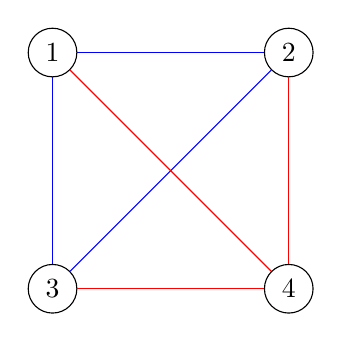
\begin{tikzpicture}[scale=3,auto=left,every node/.style={circle,draw,fill=white}]
          \node (n1) at (0,1) {1};
          \node (n2) at (1,1) {2};
          \node (n3) at (0,0) {3};
          \node (n4) at (1,0) {4};
          
          \draw [blue] (n1) -- (n2);
          \draw [blue] (n3) -- (n2);
          \draw [blue] (n1) -- (n3);
          \draw [red] (n1) -- (n4);
          \draw [red] (n2) -- (n4);
          \draw [red] (n3) -- (n4);
        \end{tikzpicture}
	\end{center}
	\caption{An image of the access structure for a $((2,4,2))$ threshold scheme, using two copies of the quantum state $\ket{\Psi}$}
	\label{fig:2-4-2}
\end{figure}

The two access structures are as follows: $\Gamma_1 = \{p_1p_2,p_2p_3,p_3p_1\}$ and $\Gamma_2 = \{p_1p_4,p_2p_4,p_3p_4\}$. Observe that each access structure satisfies is monotone and satisfies the no-cloning theorem, so a $((2,4,2))$ scheme exists. Also, note that in this scheme, it would be possible for, say, players 1 and 2 to recover the secret together \textbf{AND} players 3 and 4 to recover the secret together, and for the two pairs to do so separately. This is allowed. Each pair would recover a different copy of the state, and there is no way for the two pairs to recover the same copy, which satisfies the no-cloning theorem.

We have shown that we can implement a QTS that would otherwise not be possible in the normal construction. We call any augmented QTS that can be implemented in this way a valid scheme.

\subsection{A Graphical Representation}
\label{ssec:graphical-rep}

Our next step will be to generalize this implementation. We can start off by observing that, in the case of our $((2,4,2))$ scheme, we need the union $\Gamma_1 \cup \Gamma_2$ to consist of all subsets of size 2 from a pool of 4 players. Each of these access structures must satisfy Theorem \ref{thm:qss-disjoint}. So, in general, a $((t,n,2))$ scheme is realizable if we can take all subsets of size $t$ of the $n$ participants and divide them into $2$ groups, where each group consists of an access structure that satisfies Theorem \ref{thm:qss-disjoint}. 

Such a combinatorial problem lends itself easily to a graphical representation, albeit one that is different than the one we used above. By letting each vertex represent a player, we run into the problem where it is difficult to represent authorized sets of size greater than 2. In these cases, we would need an edge that has as its endpoints 3 or more vertices. These extensions of edges, called \textbf{hyperedges} do exist, but they would be more difficult to reason about, simply because of the lack of literature.

So, instead of representing the participants as vertices and the authorized subsets as edges between them, we take inspiration from Singh and Srikanth's AS graph representation, which we define above in \defref{defn:access-structure-graph} \cite{singh_assisted_2004}. In an AS graph, each vertex in the graph represents an authorized set, and there is an edge between two vertices if the authorized sets which they represent have a non-empty intersection. Now this is where our representation will differ slightlyfrom Singh and Srikanth. Our representation will have edges between two vertices if they \textbf{do not intersect}. In other words, we consider the \textit{complement} of the AS graph.

\begin{definition}{Access Structure Graph Complement.}
    \label{defn:access-structure-graph-complement}
	We define the \textbf{access structure graph complement} of $\Gamma$ to be the graph $G = (V,E)$, where there is a vertex $v \in V$ for each authorized subset $A \in \Gamma$. The edgeset $E$ contains an edge between each pair of vertices if their corresponding authorized subsets are disjoint.
\end{definition}

\subsection{Generalization of \texorpdfstring{$((t,n,2))$}{((t,n,2))} Schemes}
\label{ssec:generalize-t-n-2}

In the following subsection, we will explore the results that we can reach when $k=2$ by using our new formulation. The access structure graph complement for \fref{fig:2-4-2} is shown in \fref{fig:2-4-2-graph}:

\begin{figure}[H]
    \centering
	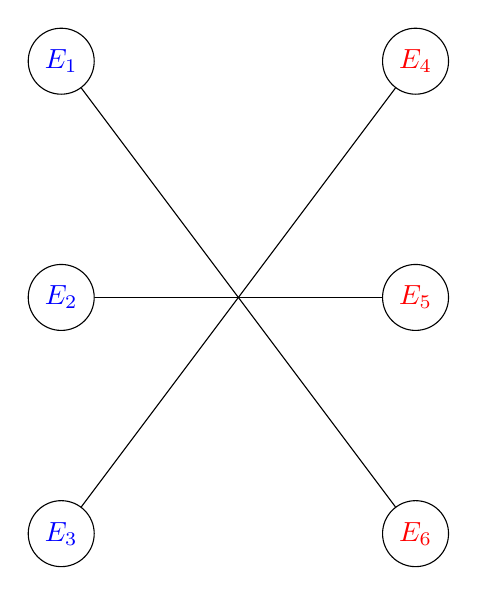
\begin{tikzpicture}[scale=3,every
	node/.style={circle,fill=white}]
      \node [draw,text=blue] (n1) at (0,3)   {$E_1$};
      \node [draw,text=blue] (n2) at (0,2)   {$E_2$};
      \node [draw,text=blue] (n3) at (0,1)   {$E_3$};
      \node [draw,text=red] (n4) at (1.5,3) {$E_4$};
      \node [draw,text=red] (n5) at (1.5,2) {$E_5$};
      \node [draw,text=red] (n6) at (1.5,1) {$E_6$};
      
      \draw [black] (n1) -- (n6);
      \draw [black] (n3) -- (n4);
      \draw [black] (n2) -- (n5);
    \end{tikzpicture}
	\caption{The access structure graph complement for a $((2,4,2))$ scheme.}
    \label{fig:2-4-2-graph}
\end{figure}

In \fref{fig:2-4-2-graph}, each vertex is an edge from \fref{fig:2-4-2}. There is an edge between the vertices if their edges are not incident to the same vertex in \fref{fig:2-4-2}. The representation illustrated in \fref{fig:2-4-2-graph} is useful to us because properties of the graph can tell us not only if a particular scheme is realizable, but why it is realizable. Let us bring in the idea of graph coloring introduced in \defref{defn:colors}.

\begin{lemma}
    \label{lem:2-color-access}
    Let a $((t,n,2))$-threshold augmented quantum secret sharing scheme have the corresponding access structure $\Gamma$. Then, this scheme is valid if and only if the access structure graph complement of $\Gamma$ is 2-colorable.
\end{lemma}

\begin{proof}
    ($\rightarrow$) Another term for 2-colorable graphs are bipartite graphs. If the AS graph of an access structure $\Gamma$ is bipartite, then we can separate the graph into two stable sets. Every pair of authorized sets in the same stable set has a non-empty intersection. So, we can assign one copy of the quantum state to each of these stable sets, and implement a QSS scheme that realizes the access structure corresponding to each particular subset of authorized sets. By construction, we have a valid augmented QTS.
    
    ($\leftarrow$) Now assume that we have a valid augmented QTS of the form $((t,n,2))$. The access structure for this scheme is $\Gamma = \Gamma_1 \cup \Gamma_2$, where $\Gamma_1$ and $\Gamma_2$ are each monotone and satisfy the no-cloning theorem. Consider just the authorized sets in $\Gamma_1$. In the AS graph complement representation, the vertices corresponding to these authorized sets must be a stable set because each pair of authorized sets in $\Gamma$ has a non-empty intersection. This is because they pairwise have a non-empty intersection. The same is true for $\Gamma_2$. Therefore, we must have a bipartite graph.
\end{proof}

By combining \lemref{lem:2-color-access} and \thmref{thm:bipartite-odd}, we get the following claim:

\begin{corollary}
    \label{cor:oddcycle-valid}
    A $((t,n,2))$ augmented QTS is valid if and only if its corresponding AS graph complement has no odd cycles.
\end{corollary}

We can use \corref{cor:oddcycle-valid} to also show that $((3,6,2))$ is also a valid scheme, but that $((2,5,2))$ and $((3,7,2))$ are \textbf{not} valid schemes.

For the $((2,5,2))$ scheme, rather than try to draw an access structure, we find an odd cycle in the AS graph complement by listing an ordering of vertices that have edges connecting them: $(1,2), (3,4), (5,1), (2,3), (4,5), (1,2)$. Each integer represents a player, and each pairing of integers represents an size-2 subset. This cycle has length 5, so the graph is not bipartite. Therefore, $((2,5,2))$ does not represent a valid augmented quantum threshold scheme. A similar approach with $((3,7,2))$ leads us to the same conclusion.

From the simple cases we have studied so far, we notice a pattern beginning to emerge. It seems like schemes of the form $((t,2t,2))$ are valid, but $((t,2t+1,2))$ are not. This turns out to be true. Using the theorems that we have developed, we will formally prove these results: that all augmented QTS of the form $((t,2t,2))$ are valid, and all augmented QTS of the form $((t, 2t+1, 2))$ are not valid. Therefore, the best that we can do with two copies of a quantum secret is $((t,2t,2))$. 

\begin{remark}
    Note that if a QTS $((t,n_1))$ is not valid because it violates the no-cloning theorem, then any QTS $((t,n_2))$ where $n_2 > n_1$ can never be valid because it must also violate the no-cloning theorem. To see this, consider the QTS $((t,n_2))$. We argue that the access structure for this scheme must be a superset of the access structure for $((t,n_1))$, if $n_2 > n_1$. In fact, we can construct the smaller access structure by selecting $n_2-n_1$ players, and removing any authrozied set with which they are associated from $\Gamma_2$ to form $\Gamma_1$.
\end{remark}

\begin{theorem}
    \label{thm:t-2t-2}
    Any augmented quantum threshold scheme of the form $((t,2t,2))$ is valid using our union of access structures strategy.
\end{theorem}

\begin{proof}
    We are given an augmented quantum threshold scheme of the form $((t,2t,2))$ where $t \geq 1$. We will show that any scheme of this form cannot have any odd cycles in its access structure graph complement. And then, by \corref{cor:oddcycle-valid}, we are done. Consider one of the authorized sets, and without loss of generality, let this set have the participants: $\{p_1,\dots,p_t\}$. Then, there is only one possible authorized set that is disjoint from this one: $\{p_{t+1},\dots,p_{2t}\}$. Note that this is true for every single authorized set (of size $t$). Therefore in the AS graph complement, each vertex has degree exactly equal to 1. Such a graph must be bipartite, and therefore cannot have any odd cycles.
\end{proof}

\begin{theorem}
    \label{thm:t-2t+1-2}
    Any augmented quantum threshold scheme of the form $((t,2t+1,2))$ is not realizable using our union of  access structures strategy.
\end{theorem}
 
\begin{proof}
    We are given an augmented quantum threshold scheme of the form $((t,2t+1,2))$ implemented over a set of players $\mathcal{P} = \{p_1,p_2,\dots,p_{2t+1}\}$, and we denote each authorized subset as an unordered set of participants. For now, assume that $t \geq 2$, because if $t=1$, the result is trivial. The only way in which we could implement a scheme over 3 players where the threshold is 1 player is to give every person a copy of the share, and we only have 2 available. 
    
    We will show that the access structure graph complement of this scheme must include an odd cycle. What we are looking for, then, is an ordered list of authorized subsets, $A_1, A_2, \dots, A_r$, such that $A_1=A_r$ and $A_i \cap A_{i+1} = \emptyset \: \forall i \in \{1,\dots,r-1\}$. If $r$ is even, then we have an odd cycle. WLOG, let the first authorized subset be $\{p_1,\dots,p_{t}\}$. From this set, we can generate a cycle of authorized sets by counting in groups of $t$ modulo $2t+1$. Here are a few of those sets in order:
    
    \begin{align*}
        &\{p_1,\dots,p_{t}\} \\ 
        &\{p_{t+1},\dots,p_{2t}\} \\ 
        &\{p_{2t+1},\dots,p_{t-1}\} \\ 
        &\{p_{t},\dots,p_{2t-1}\} \\
        & \vdots \\
        &\{p_{t+3},\dots,p_{1}\} \\ 
        &\{p_{2},\dots,p_{t+1}\} \\ 
        &\{p_{t+2},\dots,p_{2t+1}\} \\ 
        &\{p_1,\dots,p_{t}\}
    \end{align*}
    
    How many edges are in this cycle? Observe that $t$ and $2t+1$ are relatively prime, because $t \geq 2$. This means that there must be $2t+1$ edges in this cycle, which is an odd number. By \corref{cor:oddcycle-valid}, the scheme is not valid.
\end{proof}

We have shown that schemes of the form $((t,2t,2))$ are valid, but schemes of the form $((t,2t+1,2))$ are not valid. In the following chapter, we extend our results from $k=2$ to general values of $k$.





 % The Augmented Quantum Threshold Scheme

\lhead{\emph{General Augmented Quantum Secret Sharing}}
\chapter{General Results on Augmented Quantum Threshold Schemes}

\section{Generalizing the Union of Access Structures Approach}

In the previous section, we determined an upper bound on the value of $n$ with respect to $t$ at a fixed $k=2$. In this next section, we ask the question of how $n$ varies with respect to $k$, and we prove more general results about the augmented quantum threshold scheme. 

At this point, there is hardly a pattern associated with the effect of $k$, the number of copies of our quantum state, and the bounds on the values of $n$ and $t$. The approach that worked for us in the previous section was posing this problem as a graph coloring problem, and indeed, that is the approach that we will take in this section as well. Unfortunately, there does not exist a general theorem on the $c$-colorability of arbitrary graphs for $c > 3$ like there is for $2$. This problem is NP-hard. Nevertheless, it does not hurt to state clearly the following theorem:

\begin{lemma}
    \label{lem:k-color-access}
    The access structure graph complement corresponding to the augmented QTS $((t,n,k))$ is $k$-colorable if and only if $((t,n,k))$ is a valid augmented quantum threshold scheme.
\end{lemma}

This theorem and its proof are straightforward generalizations of those of \thmref{lem:2-color-access} from the previous section. In essence, the $k$-colorability of the graph ensures that we can separate it into at least $k$ stable sets, each of which can be assigned to one of the copies of the quantum state.

To continue our analysis, let us consider an example with $k=3$. Drawing on previous examples, we can show that a scheme like $((2,5,3))$ is possible. What is interesting is that this $(t,n)$ pair that would \textbf{not} be possible with $k \leq 2$. One way that we could implement this scheme would be to take our scheme for $((2,4,2))$, and add an extra copy of the state and a another player $p_5$. Then, the access structure for the newly added state contains all authorized subsets that include $p_5$. Since our original scheme was valid, then by construction, this new scheme is valid as well. We can extend this specific construction indefinitely:

\begin{theorem}
    \label{thm:build-scheme} 
    Any scheme of the form $((t,2t-2+k,k))$ is a valid augmented quantum threshold scheme.
\end{theorem}

\begin{proof}
    We have shown in \thmref{thm:t-2t-2} that schemes of the form $((t, 2t, 2))$ are realizable. Assume, as an inductive hypothesis, that $((t, 2t - 2 + i, i))$ are valid augmented quantum threshold schemes. Now, let us consider the scheme $((t, 2t-1+i, i+1))$. By our construction, we will have an access structure $\Gamma = \Gamma_1 \cup \Gamma_2 \cup ... \cup \Gamma_i \cup \Gamma_{i+1}$, where $\Gamma_r$ is the access structure corresponding to $\ket{\Psi}_r$ for $i \in {1,...,i}$. Let $\Gamma_1, ..., \Gamma_i$ remain unchanged from the scheme $((t, 2t - 2 + i, i))$. Then, we simply define $\Gamma_{i+1}$ to contain all of the authorized subsets that include the $2t-1+i$-th player. Then, this new access structure satisfies the no-cloning theorem, and by the IH, all of the access structures satisfy the no-cloning theorem. So $((t, 2t-1+i, i+1))$ is a valid augmented quantum threshold scheme.
\end{proof}

\subsection{Can we do better?}
\label{ssec:better}

\thmref{thm:build-scheme} gives us a slightly more general result, but the question still remains - can we do better? Unfortunately, the answer is in the negative. To show this result, we will bring in the Kneser Graph, introduced in \defref{defn:kneser-graph}.

\begin{remark}
    Observe that the AS graph complement of a QTS of the form $((t,n))$ is a $K(n,t)$. It is a Kneser graph on $n$ elements with subsets of size $t$. This is independent of the number of copies $k$.
\end{remark}

So, using \corref{cor:no}, we can prove the following theorem:

\begin{theorem}
    \label{thm:no-more} 
    Any scheme of the form $((t,2t-1+k,k))$ is not a valid augmented quantum threshold scheme.
\end{theorem}

\begin{proof}
    The complement of the AS graph for the access structure corresponding to the threshold scheme $((t,2t-1+k,k))$ is a $K(2t-1+k,t)$, or a Kneser Graph on a set of $2t-1+k$ elements, with subsets of size $t$. Then by \corref{cor:no}, the corresponding graph is not $k$-colorable. By \thmref{lem:k-color-access}, schemes of the form $((t,2t-1+k,k))$ are not valid augmented quantum threshold schemes.
\end{proof}

So, this is the best that we can do with $k$ copies of a quantum state, using our union of access structures approach. More specifically, we have shown that for every extra copy of the quantum state that we begin with, we are only able to implement one additional threshold scheme for a fixed group size $n$. The good news is that we have a closed form answer for the question: how many copies of the quantum state do we need to implement an augmented quantum threshold scheme $((t,n,k))$? For $n \geq 2t$, we need $k = n - 2t + 2$.

In a way, this result might be expected with our particular construction. The number of authorized sets in the access structure increases exponentially for every new person added, so it makes sense that the access structures that we can implement are constrained so tightly by the number of copies.

\section{Security Considerations}

Because we construct our scheme using a concatenation of access structures, all we need to do is show that an augmented QTS is no less secure than its constituent parts. That is, using our union of access structures strategy, if the QSS schemes that are used with each copy of the quantum state are perfect, then the resulting scheme is perfect as well.

\begin{lemma}
    \label{lem:t-2t-1}
    A quantum threshold scheme of the form $((t,2t-1))$ is a perfect quantum threshold scheme.
\end{lemma}

\begin{proof}
    The minimal authorized sets of this access structure are exactly the $t$-subsets of $2t-1$. Observe that this is a maximal access structure. The complement of any authorized set must have a size of $t-1$ or smaller. Therefore, the authorized sets are exactly the complements of the unauthorized sets, which means that this scheme is perfect. 
\end{proof}

\begin{theorem}
    An augmented QTS of the form $((t,2t-2+k,k))$ is a perfect quantum threshold scheme.
\end{theorem}

\begin{proof}
    Because our method of constructing these schemes involves a recursive structure, we can use induction to show that the entire scheme is perfect by showing that the underlying schemes that compose it are perfect. For our base case, consider the QTS $((t,2t-1))$. Note that there is an implicit $k=1$. Then by \lemref{lem:t-2t-1}.
    
    For our inductive hypothesis, assume that $((t,2t-2+k,k))$ is a perfect QTS. We will show that $((t,2t-1+k,k+1))$ is also a perfect QTS. Note that using our construction, the $((t,2t-1+k,k+1))$ is built by taking the original $((t,2t-2+k,k))$, and then adding one more share $\ket{\psi_{k+1}}$ and one more player $P_{2t-1+k}$. By the IH, we know that the smaller scheme is perfect. Therefore, we only need to show that the access structure corresponding to $\ket{\psi_{k+1}}$ is perfect. We will call this access structure $\Gamma_{k+1}$. Note that this access structure contains all of the $t$-subsets of $2t-1+k$ that contain $P_{2t-1+k}$. However, this access structure is not maximal. Namely, the subset of players $\mathcal{P} \setminus P_{2t-1+k} = \{P_1,...,P_{2t-2+k}\}$ is unauthorized, as well as its complement $\{P_{2t-1+k}\}$. However, we can construct this access structure out of maximal access structures using a construction presented by Gottesman in \cite{gottesman_theory_2000}.
    
    First, let the maximal access structure containing $\Gamma_{k+1}$ be $\Gamma^M$. Then, $\Gamma_M = \Gamma_{k+1} \cup \{P_1,...,P_{2t-2+k}\}$. This is both a minimal and maximal access structure. It contains only minimal authorized sets, but the authorized sets are exactly the complements of the unauthorized sets. Let's denote the number of minimal authorized sets in $\Gamma^M$ to be $r$. $r = \binom{t}{2t-1+k} + 1$. Then, we construct a layered scheme, using a $((r,2r-1))$ scheme. Let the shares of this scheme be $S_i$ for $i \in \{1,...,2r-1\}$. For the first $r$ shares, we use a secret sharing scheme to divide shares among the authorized set. The schemes are $((l_i,l_i))$ threshold schemes, where $l_i = |A_i|$ is the size of the corresponding authorized set. The latter $r-1$ shares all have access structure equal to $\Gamma^M$. In this way, Any access structure $A_1,\dots,A_r$ will be able to recover one of the first $r$ shares, and will also be able to recover the latter $r-1$ shares. This allows that authorized set to recover the secret. However, an authorized set that is in $\Gamma^M$ but not in $\Gamma$ cannot recover enough shares to recover secret. 
    
    Note that any scheme of the form $((r,2r-1))$ is maximal, as is any scheme of the form $((t,t))$. The authorized sets are the complements of the unauthorized sets. So, we have found a way to construct $\Gamma_{k+1}$ using only maximal access structures. Therefore, $\Gamma_{k+1}$ is a perfect secret sharing scheme, so by induction $((t,2t-2+k,k))$ is a perfect quantum threshold scheme.
\end{proof}

\section{Assisted Quantum Secret Sharing and Augmented Quantum Secret Sharing}
\label{sec:aqss-and-aqss}

In this section, we give a short result on that provides a closed form solution for the number of resident shares needed in an assited QSS implementation of a threshold scheme. Recall the assisted quantum secret sharing scheme presented by Singh and Srikanth \cite{singh_assisted_2004}. They show that, by using a system of resident shares and player shares, they are able to realize any quantum secret sharing scheme corresponding to a monotone access structure. The number of resident shares needed is $\lambda-1$, where $\lambda$ is the minimum number of partially linked classes there are in the AS graph of the access structure $\Gamma$. The question that is left open is finding a way to compute $\lambda$. Using the following proposition, we show that our results from the previous section can provide a closed form answer to this question when the access structure corresponds to a threshold scheme.

Let us consider a quantum threshold scheme $((t,n))$. How many resident shares are needed to realize this scheme? By \propref{prop:chrom-clique}, the minimum number of partially linked classes in the AS graph is the same as the chromatic number of the AS graph's complement. So, by Kneser's Conjecture, finding this for quantum threshold schemes is easy. The AS graph complement of this scheme is a Kneser graph on $n$ elements with subsets of size $t$. The chromatic number of the AS graph complement is $n-2t+2$, so $\lambda = n-2t+2$. Therefore, the minimum number of resident shares we need for an assisted quantum threshold scheme on $n$ players with threshold $t$ is $n-2t+1$. % The General Results

\lhead{\emph{Conclusion}}
\chapter*{Conclusion}
\label{conclusion}

We have shown that  % Conclusion

%% ----------------------------------------------------------------
% Now begin the Appendices, including them as separate files

\addtocontents{toc}{\vspace{2em}} % Add a gap in the Contents, for aesthetics

\appendix % Cue to tell LaTeX that the following 'chapters' are Appendices

%\chapter{An Appendix}

Lorem ipsum dolor sit amet, consectetur adipiscing elit. Vivamus at pulvinar nisi. Phasellus hendrerit, diam placerat interdum iaculis, mauris justo cursus risus, in viverra purus eros at ligula. Ut metus justo, consequat a tristique posuere, laoreet nec nibh. Etiam et scelerisque mauris. Phasellus vel massa magna. Ut non neque id tortor pharetra bibendum vitae sit amet nisi. Duis nec quam quam, sed euismod justo. Pellentesque eu tellus vitae ante tempus malesuada. Nunc accumsan, quam in congue consequat, lectus lectus dapibus erat, id aliquet urna neque at massa. Nulla facilisi. Morbi ullamcorper eleifend posuere. Donec libero leo, faucibus nec bibendum at, mattis et urna. Proin consectetur, nunc ut imperdiet lobortis, magna neque tincidunt lectus, id iaculis nisi justo id nibh. Pellentesque vel sem in erat vulputate faucibus molestie ut lorem.

Quisque tristique urna in lorem laoreet at laoreet quam congue. Donec dolor turpis, blandit non imperdiet aliquet, blandit et felis. In lorem nisi, pretium sit amet vestibulum sed, tempus et sem. Proin non ante turpis. Nulla imperdiet fringilla convallis. Vivamus vel bibendum nisl. Pellentesque justo lectus, molestie vel luctus sed, lobortis in libero. Nulla facilisi. Aliquam erat volutpat. Suspendisse vitae nunc nunc. Sed aliquet est suscipit sapien rhoncus non adipiscing nibh consequat. Aliquam metus urna, faucibus eu vulputate non, luctus eu justo.

Donec urna leo, vulputate vitae porta eu, vehicula blandit libero. Phasellus eget massa et leo condimentum mollis. Nullam molestie, justo at pellentesque vulputate, sapien velit ornare diam, nec gravida lacus augue non diam. Integer mattis lacus id libero ultrices sit amet mollis neque molestie. Integer ut leo eget mi volutpat congue. Vivamus sodales, turpis id venenatis placerat, tellus purus adipiscing magna, eu aliquam nibh dolor id nibh. Pellentesque habitant morbi tristique senectus et netus et malesuada fames ac turpis egestas. Sed cursus convallis quam nec vehicula. Sed vulputate neque eget odio fringilla ac sodales urna feugiat.

Phasellus nisi quam, volutpat non ullamcorper eget, congue fringilla leo. Cras et erat et nibh placerat commodo id ornare est. Nulla facilisi. Aenean pulvinar scelerisque eros eget interdum. Nunc pulvinar magna ut felis varius in hendrerit dolor accumsan. Nunc pellentesque magna quis magna bibendum non laoreet erat tincidunt. Nulla facilisi.

Duis eget massa sem, gravida interdum ipsum. Nulla nunc nisl, hendrerit sit amet commodo vel, varius id tellus. Lorem ipsum dolor sit amet, consectetur adipiscing elit. Nunc ac dolor est. Suspendisse ultrices tincidunt metus eget accumsan. Nullam facilisis, justo vitae convallis sollicitudin, eros augue malesuada metus, nec sagittis diam nibh ut sapien. Duis blandit lectus vitae lorem aliquam nec euismod nisi volutpat. Vestibulum ornare dictum tortor, at faucibus justo tempor non. Nulla facilisi. Cras non massa nunc, eget euismod purus. Nunc metus ipsum, euismod a consectetur vel, hendrerit nec nunc.	% Appendix Title

\addtocontents{toc}{\vspace{2em}}  % Add a gap in the Contents, for aesthetics
\backmatter

%% ----------------------------------------------------------------
\label{Bibliography}
\lhead{\emph{Bibliography}}  % Change the left side page header to "Bibliography"
\bibliographystyle{unsrtnat}  % Use the "unsrtnat" BibTeX style for formatting the Bibliography
\bibliography{Bibliography}  % The references (bibliography) information are stored in the file named "Bibliography.bib"

\end{document}  % The End
%% ----------------------------------------------------------------